%!TEX root = ../thesis.tex
本研究で開発するオフィスロボットは,従来のオフィスロボットが取り組んでいる作業を基に,特定の代表的な作業に焦点を当てる.本章では,開発するオフィスロボットが対象とする作業を決定し,その作業に必要なロボットアームのメカニズム要件について述べる.
\section{作業調査}
対象とする作業は,従来のオフィスロボットが行っている作業を参考に決定する.
オフィスロボットが行っている作業事例を動画や文献から合計77件抽出したところ,約61\%が台車移動とピック\&プレイスを組み合わせた作業であった.例えば,部屋の片づけや荷物の運搬などが代表例である.その他の作業は,ドアの開閉,ボタンの押下,フロアの巡回,などが見られた.

以上の結果から,現在オフィスロボットが対象としている作業の多くは,物体を把持して移動させる作業であることがわかる.そこで,本研究では「机の片づけ作業」を対象とする.これを選定した理由は以下の3点である.
\begin{itemize}
  \item 片づけ作業は,オフィス環境において頻出する基本的なタスクである
  \item 多様な形状・サイズの物体を扱うため,ロボットアームの性能評価に適している
  \item 実用化に向けた汎用性が高く,他の作業へ応用しやすい
\end{itemize}

\section{作業詳細}
机の片づけ作業は,机の上に散らばっている物体を事前に設置した箱の中へ移動させる作業である.本節では,具体的に使用する物体の種類,サイズ,重量,設置位置について述べる.
\subsection{種類}
ロボットが把持対象とする物体は,従来のオフィスロボットが頻繁に把持していた物体を調査したうえで設定した.図\ref{fig:handget}に示すように,最も多かったのは服やタオルなどの衣類で,次にペットボトルや缶ジュースなどの筒状物,お菓子の箱や 200ml 程度のパックジュースなどの箱状物,さらにペンなどの棒状物や雑誌などの薄型物が続いた.これらの結果に基づき,本研究ではハンドタオル,缶ジュース,パックジュースの 3 種類を使用する.
\begin{figure}[h]
  \centering
  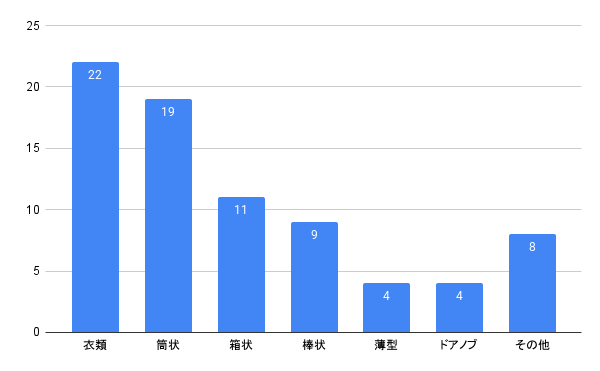
\includegraphics[width=10cm]{images/2syou/handget.png}
  \caption{Survey results of objects grasped by office robots}
  \label{fig:handget}
\end{figure}
\clearpage
\subsection{サイズと重量}
調査の中では,人が片手で持てないサイズや重量の大きい物体を扱う事例は見られなかった.また,対象物として設定した缶ジュースやパックジュースの平均的なサイズと重量は,幅6~8cm,重量300~400g程度であった.これに基づき,本研究では対象物の幅を10cm以下,重量を500g以下と設定した.
\subsection{設置位置}
把持対象物と箱の設置位置は,従来のオフィスロボットのアームリーチに基づいて設定した.調査では,Hello Robot社が開発したStretch 3のアームリーチが約0.51mであり,これが現行ロボットの最小リーチ値であることが確認された.このため,本研究では把持対象物と箱の設置位置を机の縁から0.5m以内の範囲とする.
\newpage